%%%%%%%%%%%%%%%%%%%%%%%%%%%%%%%%%%%%%%%%%
% Short Sectioned Assignment LaTeX Template Version 1.0 (5/5/12)
% This template has been downloaded from: http://www.LaTeXTemplates.com
% Original author:  Frits Wenneker (http://www.howtotex.com)
% License: CC BY-NC-SA 3.0 (http://creativecommons.org/licenses/by-nc-sa/3.0/)
%%%%%%%%%%%%%%%%%%%%%%%%%%%%%%%%%%%%%%%%%

%----------------------------------------------------------------------------------------
%	PACKAGES AND OTHER DOCUMENT CONFIGURATIONS
%----------------------------------------------------------------------------------------

\documentclass[paper=a4, fontsize=11pt]{scrartcl} % A4 paper and 11pt font size

% ---- Entrada y salida de texto -----

\usepackage{hyperref}
\usepackage{listings}
\usepackage{color}
%AÑADIDO DE LA PÁGINA http://stackoverflow.com/questions/3175105/how-to-insert-code-into-a-latex-doc
\definecolor{dkgreen}{rgb}{0,0.6,0}
\definecolor{gray}{rgb}{0.5,0.5,0.5}
\definecolor{mauve}{rgb}{0.58,0,0.82}

\lstset{frame=tb,
	language=Python,
	aboveskip=3mm,
	belowskip=3mm,
	showstringspaces=false,
	columns=flexible,
	basicstyle={\small\ttfamily},
	numbers=none,
	numberstyle=\tiny\color{gray},
	keywordstyle=\color{blue},
	commentstyle=\color{dkgreen},
	stringstyle=\color{mauve},
	breaklines=true,
	breakatwhitespace=true,
	tabsize=3
}
%%%%%%%%%%%%%%%%%%%%%%%%%%%%%%%%%%%%%%%%%%%%%%%%%%%%%%%
\usepackage{varioref}
\usepackage[T1]{fontenc} % Use 8-bit encoding that has 256 glyphs
\usepackage[utf8]{inputenc}
%\usepackage{fourier} % Use the Adobe Utopia font for the document - comment this line to return to the LaTeX default

% ---- Idioma --------

\usepackage[spanish, es-tabla]{babel} % Selecciona el español para palabras introducidas automáticamente, p.ej. "septiembre" en la fecha y especifica que se use la palabra Tabla en vez de Cuadro

% ---- Otros paquetes ----

\usepackage{amsmath,amsfonts,amsthm} % Math packages
%\usepackage{graphics,graphicx, floatrow} %para incluir imágenes y notas en las imágenes
\usepackage{graphics,graphicx, float} %para incluir imágenes y colocarlas

% Para hacer tablas comlejas
%\usepackage{multirow}
%\usepackage{threeparttable}

%\usepackage{sectsty} % Allows customizing section commands
%\allsectionsfont{\centering \normalfont\scshape} % Make all sections centered, the default font and small caps

\usepackage{fancyhdr} % Custom headers and footers
\pagestyle{fancyplain} % Makes all pages in the document conform to the custom headers and footers
\fancyhead{} % No page header - if you want one, create it in the same way as the footers below
\fancyfoot[L]{} % Empty left footer
\fancyfoot[C]{} % Empty center footer
\fancyfoot[R]{\thepage} % Page numbering for right footer
\renewcommand{\headrulewidth}{0pt} % Remove header underlines
\renewcommand{\footrulewidth}{0pt} % Remove footer underlines
\setlength{\headheight}{13.6pt} % Customize the height of the header

\numberwithin{equation}{section} % Number equations within sections (i.e. 1.1, 1.2, 2.1, 2.2 instead of 1, 2, 3, 4)
\numberwithin{figure}{section} % Number figures within sections (i.e. 1.1, 1.2, 2.1, 2.2 instead of 1, 2, 3, 4)
\numberwithin{table}{section} % Number tables within sections (i.e. 1.1, 1.2, 2.1, 2.2 instead of 1, 2, 3, 4)

\setlength\parindent{0pt} % Removes all indentation from paragraphs - comment this line for an assignment with lots of text

\newcommand{\horrule}[1]{\rule{\linewidth}{#1}} % Create horizontal rule command with 1 argument of height


\renewcommand{\reftextbefore}
	{en la  \reftextvario{página que precede a esta}{página anterior}}
\renewcommand{\reftextafter}
	{en la \reftextvario{siguiente}{siguiente} página}
\renewcommand{\reftextfacebefore}
	{en la  \reftextvario{anterior}{anterior} página}
\renewcommand{\reftextfaceafter}
	{en la \reftextvario{siguiente}{siguiente}{página}}

 \usepackage{algpseudocode}
%----------------------------------------------------------------------------------------
%	TÍTULO Y DATOS DEL ALUMNO
%----------------------------------------------------------------------------------------

\title{	
\normalfont \normalsize 
\textsc{{\bf Algorítmica (2015-2016)} \\ Grado en Ingeniería Informática \\ Universidad de Granada} \\ [25pt] % Your university, school and/or department name(s)
\horrule{0.5pt} \\[0.4cm] % Thin top horizontal rule
\huge Práctica 4-Primera Parte: Cena de gala \\ % The assignment title
\horrule{2pt} \\[0.5cm] % Thick bottom horizontal rule
}

\author{Francisco Carrillo Pérez,Borja Cañavate Bordons, \\Miguel Porcel Jiménez,Jose Manuel Rejón Santiago,Jose Arcos Aneas} % Nombre y apellidos

\date{\normalsize\today} % Incluye la fecha actual

%----------------------------------------------------------------------------------------
% DOCUMENTO
%----------------------------------------------------------------------------------------

\begin{document}

\maketitle % Muestra el Título

\newpage %inserta un salto de página

\tableofcontents % para generar el índice de contenidos

\listoffigures

\listoftables

\newpage

\section{Introducción }

El objetivo de esta práctica es diseñar un algoritmo Backtracking, que resuelva uno de los cinco problemas de la práctica y realizar un estudio empírico de su eficiencia.
	
	Se desea sentar a N invitados alrededor de una mesa, de manera que cada invitado tendra a su lado a otros dos. Cada par de invitados tiene un nivel de compatibilidad. Se desea maximizar la compatibilidad de estos comensales.
%----------------------------------------------------------------------------------------

	

%------------------------------------------------------------------------------------------

\section{Elementos de la solución al problema}

	Dada una matriz M[i][j] 
	Mantenemos en la matriz la afinidad  entre 
	el comensal i y el comensal j
	
	
	\[ \left( \begin{array}{ccc}
	0 & 30 & 15 \\
	30 & 0 & 20 \\
	15 & 20 & 0 \end{array} \right)\] 



\subsection{Representación de la compatibilidad}
La entrada sera una matriz simetrica de valores aleatorios con la diagonal de 0s.

\subsection{Representación de la solución}
Vector de longitud igual al número de invitados (\textit{N}), en que cada posición guarda el valor del invitado que se sienta en la posición \textit{i}.

\subsection{Solucion parcial}
olucion parcial al problema de tamaño menor que N.


\subsection{Restricciones explícitas}
Los valores que puede tomar la solucion son los enteros de 1 a N. Donde N es el número total de invitados. 

\subsection{Restricciones implícitas}
Estas restricciones son las que determinan si una función parcial puede llevarnos a una solucion del problema. Si supera un umbral. 


%--------------------------------------------------------------------------------------------

\section{Pseudocódigo}

\begin{algorithmic}				
	\Require Matriz, S\_final[N] S\_parcial[N] Sentados[N]={false} comensal\_actual, nivel,valor\_maximo=0;
	\State \textbf{Funcion(S,S\_parcial,Sentados,comensal\_actual,nivel):}
	\State Sentados[comensal\_actual]=true;
	\State	   S\_parcial[nivel - 1]=comensal\_actual;
	\For {\textbf{i} to \textbf{N}}
	
	\If {Sentados[i]==false}
	\State 	valor\_actual = CalcularSolucionActual(S\_parcial);
	\State 	\textbf{Funcion(S,S\_parcial,Sentados,i,nivel+1);}
	\If{nodo\_actual == nodo\_hoja}
	\State{ valor\_actual = CalcularSolucionActual()}
	\If{valor\_actual \textbf{mayor que} valor\_maximo)}
	\State{ S\_final = S\_Actual}
	\State{ valor\_maximo = valor\_actual}
	\EndIf
	\EndIf
	
	\State Sentados[i] = false;
	\EndIf
	\EndFor
	
	
\end{algorithmic}	


\section{Eficiencia}




	
	\begin{figure}[H]
		\centering
		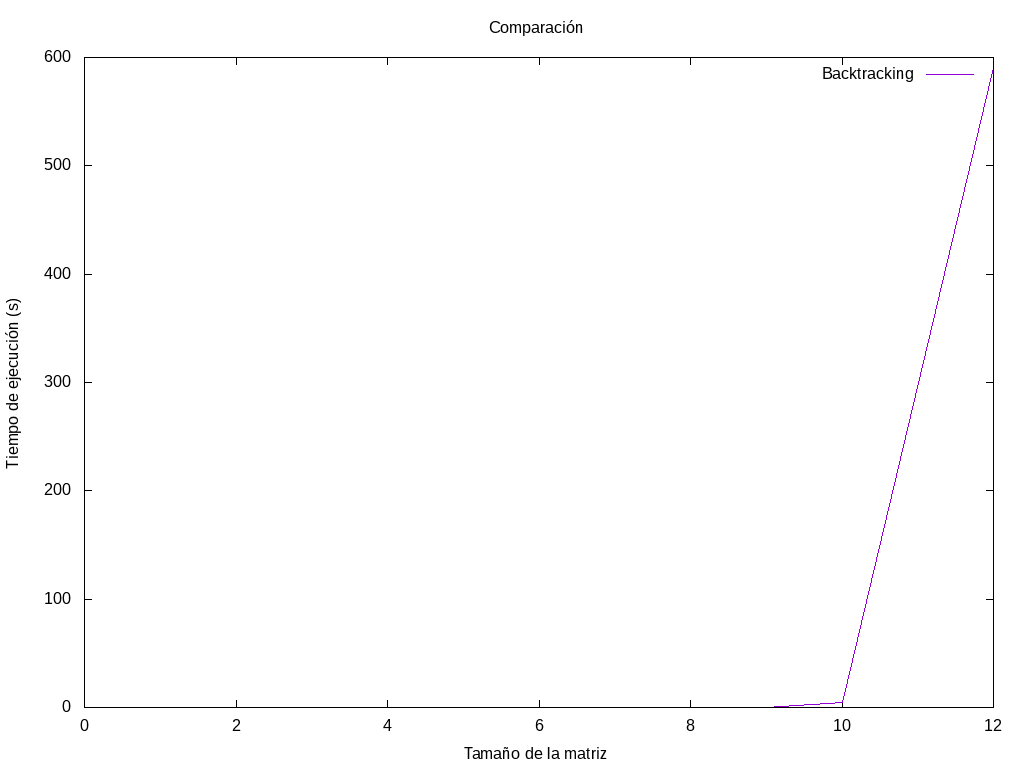
\includegraphics[width=0.7\linewidth,scale=1.5]{../Codigo/backtrackempirica}
		\caption{algoritmo backtracking}
		\label{fig:backtrackhibrida}
	\end{figure}
	
	

\subsection{Eficiencia Híbrida}	
	
	\begin{figure}[H]
		\centering
		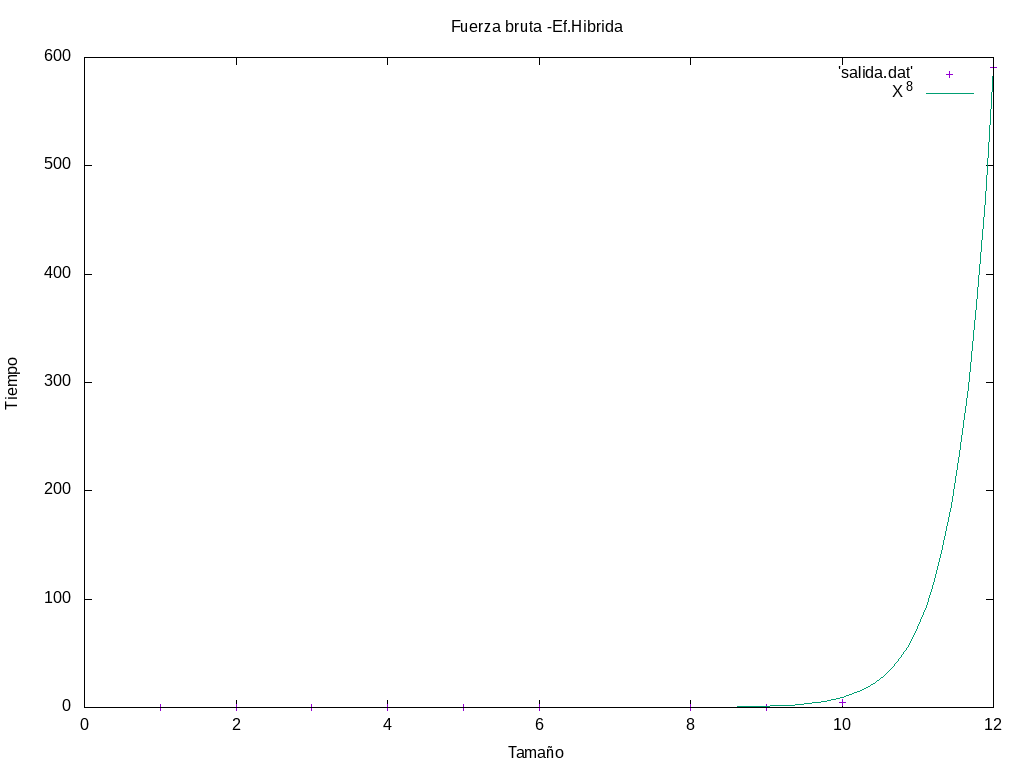
\includegraphics[width=0.7\linewidth,scale=1.5]{../Codigo/backtrackhibrida}
		\caption{comparación x**8 vs algoritmo backtracking}
		\label{fig:backtrackhibrida}
	\end{figure}
	

	Ajuste con X**8
	
	\begin{table}[H]
		\centering
		\caption{Ef híbrida obtenida}
		\label{my-label}
		\begin{tabular}{lll}
			& Final set of parameters &   Asymptotic Standard Error & \\
			& a0  = 8.59555e-09 &  +/- 2.326e-11    (0.2706\%)&  \\
			
		\end{tabular}
	\end{table}
	




\end{document}